\documentclass[a4paper,12pt]{article}
\usepackage{amsmath, amsthm, amssymb}
\usepackage{datetime}
\usepackage{framed}
\usepackage{enumitem}
\usepackage{fancyref}
\usepackage{wrapfig}
\usepackage{pifont}

\usepackage{csquotes}
\renewcommand{\mkbegdispquote}[2]{\itshape}

\newcommand{\longcaption}[2]{\caption[#1]{\textbf{#1}:#2}}

\usepackage{data/circledsteps}
\usepackage[top=1in,bottom=1in,left=1in,right=1in]{geometry} % 用于设置页面布局
\usepackage{xeCJK} % 用于使用本地字体
\usepackage[super, square, sort&compress]{natbib} % 处理参考文献
\usepackage{titlesec, titletoc} % 设置章节标题及页眉页脚
%\usepackage{xCJKnumb} % 中英文数字转换
\usepackage{amssymb}
\usepackage{amsmath} % 在公式中用\text{文本}输入中文
\usepackage{diagbox}
\usepackage{multirow} % 表格中使用多行
\usepackage{booktabs} % 表格中使用\toprule等命令
\usepackage{rotating} % 使用sidewaystable环境旋转表格
\usepackage{tabularx}
\usepackage{graphicx} % 处理图片
\usepackage{footnote} % 增强的脚注功能,可添加表格脚注
\usepackage{threeparttable} % 添加真正的表格脚注,示例见README
\usepackage{hyperref} % 添加pdf书签

\usepackage{tikz}
\usetikzlibrary{shapes,arrows,shadows}

% 字体设置
\setmainfont{Times New Roman}
\setsansfont[Scale=MatchLowercase,Mapping=tex-text]{PT Sans}
\setmonofont[Scale=MatchLowercase]{PT Mono}
\setCJKmainfont[ItalicFont={Kaiti SC}, BoldFont={Heiti SC}]{Songti SC}
\setCJKsansfont{Heiti SC}
\setCJKmonofont{Songti SC}
% \setCJKmainfont[BoldFont={FZXiaoBiaoSong-B05S}]{Songti SC}
% \setCJKfamilyfont{kai}[BoldFont=Heiti SC]{Kaiti SC}
% \setCJKfamilyfont{song}[BoldFont=Heiti SC]{Songti SC}
% \setCJKfamilyfont{hei}[BoldFont=Heiti SC]{Heiti SC}
% \setCJKfamilyfont{fsong}[BoldFont=Heiti SC]{Songti SC}
% \newcommand{\kai}[1]{{\CJKfamily{kai}#1}}
% \newcommand{\hei}[1]{{\CJKfamily{hei}#1}}
% \setromanfont[Mapping=tex-text]{TeXGyrePagella}
% \setsansfont[Scale=MatchLowercase,Mapping=tex-text]{TeXGyrePagella}
% \setmonofont[Scale=MatchLowercase]{Courier New}
%%设置常用中文字号,方便调用
\newcommand{\erhao}{\fontsize{22pt}{\baselineskip}\selectfont}
\newcommand{\xiaoerhao}{\fontsize{18pt}{\baselineskip}\selectfont}
\newcommand{\sanhao}{\fontsize{16pt}{\baselineskip}\selectfont}
\newcommand{\xiaosanhao}{\fontsize{15pt}{\baselineskip}\selectfont}
\newcommand{\sihao}{\fontsize{14pt}{\baselineskip}\selectfont}
\newcommand{\xiaosihao}{\fontsize{12pt}{\baselineskip}\selectfont}
\newcommand{\wuhao}{\fontsize{10.5pt}{\baselineskip}\selectfont}
\newcommand{\xiaowuhao}{\fontsize{9pt}{\baselineskip}\selectfont}
\newcommand{\liuhao}{\fontsize{7.5pt}{\baselineskip}\selectfont}

% 章节标题显示方式及页眉页脚设置
% \item xCJKnumb是自己额外安装的包
% \item titleformat命令定义标题的形式
% \item titlespacing定义标题距左、上、下的距离
\titleformat{\section}{\raggedright\large\bfseries}{\thesection}{1em}{}
\titleformat{\subsection}{\raggedright\normalsize\bfseries}{\thesubsection}{1em}{}
\titlespacing{\section}{0pt}{*0}{*2}
\titlespacing{\subsection}{0pt}{*0}{*1}
% 由于默认的2em缩进不够,所以我手动调整了,但是在windows下似乎2.2就差不多了,或者是article中没有这个问题
\setlength{\parindent}{2.2em}

% 设置表格标题前后间距
\setlength{\abovecaptionskip}{0pt}
\setlength{\belowcaptionskip}{0pt}


\renewcommand{\refname}{\bfseries{参~考~文~献}} %将Reference改为参考文献(用于 article)
% \renewcommand{\bibname}{参~考~文~献} %将bibiography改为参考文献(用于 book)
\renewcommand{\baselinestretch}{1.38} %设置行间距
\renewcommand{\figurename}{\small\ttfamily 图}
\renewcommand{\tablename}{\small\ttfamily 表}


\title{大脑如何制造混沌以理解世界}
\date{1987 年}
\author{Christine A. Skarda\\Walter J. Freeman}

\begin{document}

\maketitle{}
\centerline{ ChatGPT (译) }
\centerline{ 苑明理 (校) }
\centerline{\rule{14cm}{0.4pt}}
\begin{displayquote}
近期的“连接主义”模型为理解大脑功能提供了一种新的解释性选择,与传统的数字计算机模型形成对比。我们对嗅球的脑电图研究显示,大脑可能确实采用了类似于连接主义模型中的计算机制。本文中,我们探讨了我们的研究数据,并发展了一个模型来描述负责气味识别和辨别的神经动力学。研究结果指出,在脑电图活动的空间维度中存在与感觉和运动特定的信息,并且需要新的生理学隐喻和分析技术。我们的模型特别强调混沌神经活动的重要性。我们假设混沌行为是神经感知系统的基本状态,并提出了一种机制,用于学习对应于新气味的有规律的活动模式。最后,我们简要讨论了这个神经模型对行为理论的一些潜在影响。我们的研究与连接主义的工作共同促使我们重新评估那些仅基于数字计算机隐喻的解释模型。

关键词:大脑理论;混沌;认知主义;连接主义;脑电图;非线性动力学;嗅觉;感知;感觉
\end{displayquote}

\centerline{\rule{14cm}{0.4pt}}

\section{引言}

要理解大脑的功能,我们必须明白感觉系统是如何处理信息的。近期的连接主义模型相对于早期基于数字计算机的信息处理模型提供了一个新颖的解释途径,这些早期模型认为神经元是以两种状态进行逻辑决策的元素,通过网络组织起来计算简单的布尔函数。在这篇文章中,我们将总结我们实验室的一些实验结果,这些结果显示在中枢神经系统的脑电图活动的空间维度中存在与感觉和运动相关的特定信息。基于我们的数据,我们构建了一个解释性模型,描述了负责感觉编码的神经状态;这个模型与模仿数字计算机的传统模型有显著的不同,并在计算原则上与最近的连接主义模型有所吻合。我们认为,大脑依赖于一些在其他模型中未出现的机制;我们提出了四种可能对于在充满不可预测和频繁剧烈变化的环境中适应性行为的系统的有效运作和生存至关重要的机制。
我们的模型特别强调了大脑活动中的“混沌”现象。我们认为大脑依靠混沌活动而非稳定或随机活动来实现多个目标:混沌是所有感知过程中基本的集体神经活动形式,它既是一种受控制的噪声源,也是确保持续接触到以前学习的感觉模式的手段,同时也是学习新的感觉模式的方法。

\section{方法论考虑}

感觉系统是如何处理信息的呢?基于数字计算机的模型定义了计算为一种物理操作,由系统部件的子状态控制,这些子状态根据规则操作符号标记的形式句法结构而定义,与系统中的实际物理差异相对应。这些形式元素或符号必须是离散的——也就是说,它们独立于上下文;每一个不同的语义特性必须与一个不同的物理特性相关联\cite[p.~50,74]{pylyshyn1984}。

多年来,生理学家在解读他们的数据时已经应用了计算模型。因此,他们发现外围感觉系统的“编码”基于“标记线”\cite[p.~274]{bullock1965};刺激的性质是通过选择一个或多个从众多可用轴突中的轴突来传达的,而强度则是通过每个轴突上每单位时间的动作电位数量来传达的。这个模型对于外周运动系统和中枢神经系统的某些部分是有效的,尤其是在能够识别“特征检测器”和“指令”神经元的情况下。然而,在中枢联合功能的信息处理模式的研究中并未取得成功\cite{barlow1972}\cite{perkel1968}。

我们尝试理解嗅觉中的信息处理是基于三个基本假设。首先,当一个动物经过训练能够区分两种气味刺激,并且吸入其中之一(即条件刺激[CS])然后做出正确的反应(即条件反应[CR])时,在CS和CR的开始之间的某个时刻,嗅球中会存在与特定气味相关的信息,作为做出正确CR的基础。其次,这些信息将被编码为每种气味CR对应的空间-时间神经活动模式。第三,这些模式将以某种方式间接地在嗅球表面记录的脑电图潜在活动中体现出来。经过12年的研究,我们最终确认了一些预设的模式\cite{freeman1986a}。这些结果令人非常惊讶;它们让我们的认识远远超出了之前的预期,以至于我们找不到合适的生理学比喻来描述它们,不得不借鉴一些新兴的、引人入胜的数学和物理学领域来理解它们的意义。

从原理上说,这些实验非常简单。口渴的兔子被训练\cite{prisco1985},以在闻到一种特定气味(条件刺激,CS+)时舔水(条件反应,CR+),该气味在2秒后会伴随水的给予,而对于另一种未强化的气味(条件刺激,CS-),它们只是进行简单的嗅闻(条件反应,CR-)。每只兔子的左侧嗅球表面永久植入了64个电极的阵列。这64条脑电图信号被放大、过滤,并在每次试验中的短时间内进行测量;在采取了适当的保护措施\cite{freeman1987b}后,这些来自多次试验的测量数据被用来将脑电图的时期分为不同的组,与CS和CR相关。特定于气味的信息被发现存在于所有64个通道共有的脑电图电位振荡波形的幅度空间模式中,由此推断整个嗅球也是如此。我们得出结论,嗅球中的每个神经元都参与了每一个嗅觉区分反应,因为它们都参与了这种振荡。区分不同气味EEG模式的唯一因素是在共同频率上,事件时间窗口内平均强度的空间配置,就像单色光模式通过灰度来区分一样。在64条轨迹中的局部相位变化、幅度调制、频率调制及其它方面,并没有发现包含特定于气味的信息。

关于我们的第一个假设(嗅球中必须存在与特定气味相关的信息),我们选择研究嗅觉系统是因为它是最简单、进化上最稳定和最具代表性的感觉系统,其结构和功能也是最为人所了解的。此外,研究嗅觉系统的早期阶段无需直接涉及脑干和丘脑。我们选择兔子作为实验对象,因为它的头部足够大,可以支撑长期植入和64个通道的电连接器,而且其嗅球足够小,电极阵列可以覆盖其表面的相当大部分(在兔子中约占20\%,相对于猫的6\%;\cite{freeman1978})。我们采用食欲条件反射,以便从每只动物身上观察到可区分的行为反应:对CS+(条件刺激+)的反应是舔水,伴有或不伴有嗅闻(CR+),而对CS-(条件刺激-)的反应则仅为嗅闻(CR-)。我们发现,这些自然形成的条件反应(自发的运动活动模式)在第一次会话的几次试验中就出现了较高的相对发生频率,它们在多次会话中保持稳定,并且可以轻松且可靠地进行定量分析\cite{freeman1981} \cite{freeman1986b}。

\section{神经生理学结果}

\begin{figure}[ht]
    \centering
    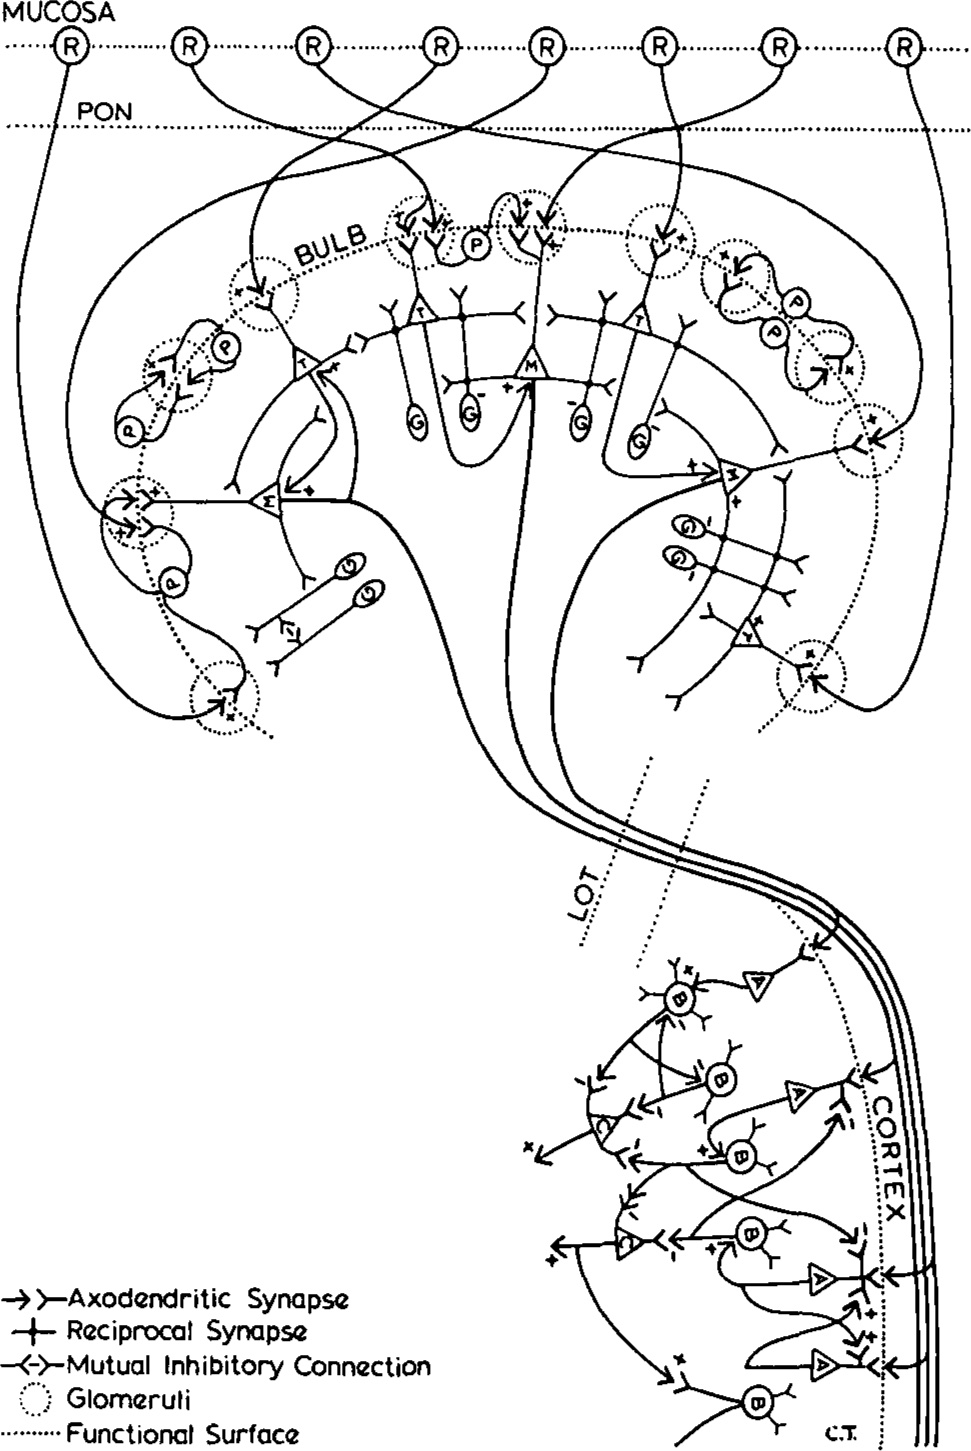
\includegraphics[height=5.5in]{images/fig1.jpg}
    \longcaption{嗅球和前梨状皮层中主要细胞类型及其相互连接的示意图}{R代表受体;PON表示初级嗅神经;LOT为侧嗅道;M为颗粒细胞;P为围葡萄状细胞;A为表层锥形细胞;B也代表颗粒细胞;C为深层锥形细胞。摘自 Freeman (1972)。}
\end{figure}

\subsection{神经活动的空间分析}

就我们的第二个假设而言(特定于气味的信息以时空活动模式编码),鼻中的化学感受器神经元集合和它们在嗅球中投射轴突的颗粒细胞集合(见图1)都呈片状分布。受体单位活动、电嗅图以及气味剂刺激时黏膜的气味吸收测量显示,对特定气味剂敏感的受体细胞在黏膜中分布不均,它们的空间激活模式随气味剂不同而有所差异(参见Moulton 1976;Freeman \& Skarda 1985的综述)。初级嗅神经(PON)在嗅球上的投射具有一定程度的全息地图顺序。使用2-脱氧葡萄糖(2-DOG)在嗅球中的积累的研究表明,在暴露于气味剂45分钟后,嗅球外层(葡萄状层)中的密集斑块不均匀聚集,这表明受体活动的空间模式可能在嗅球内产生一个神经活动的空间模式,进而可能将特定于气味的信息传递给嗅皮层。然而,代谢研究无法揭示这种神经活动在0.1秒这样的短时间内的动态形态。

关于我们的第三个假设(特定于气味的信息在脑电图中得以体现),在受体层、嗅球和皮层中,单个神经元对于不同浓度的气味剂测试阵列有选择性的反应。在整个嗅觉系统的所有环节中,涉及多种气味剂的反应特征的变化性和重叠程度都很高,没有迹象显示更靠近中心的神经元比受体对气味剂有更“狭窄的调谐”。类似于颜色或味觉的“基本气味”的数量甚至是否存在都是未知的。

我们早期尝试展示嗅球单元对气味剂反应的空间模式是基于10个微电极同时进行的多单元胞外记录;但这种空间采样太小,且收集样本所需的时间(几分钟)过长。我们转而使用从嗅球表面的脑电图记录,因为我们发现嗅球表面特定点上的EEG电位幅度与位于这些点下方几百微米的颗粒细胞和凸起细胞的放电率之间存在密切的时间和空间统计关系。也就是说,表面的EEG(见图2),主要由嗅球深处的主要抑制性中间神经元——颗粒细胞的细胞外复合突触后电位组成(见图1),提供了对局部平均颗粒细胞活动模式的间接访问,这些活动模式构成了嗅球对嗅皮层的输出。关于这一推论的理论和实验证据,包括体积传导理论和嗅球神经元动力学的研究,已在一本专著(Freeman 1975)中进行了汇编,感兴趣的读者可以参阅。

\begin{figure}[ht]
    \centering
    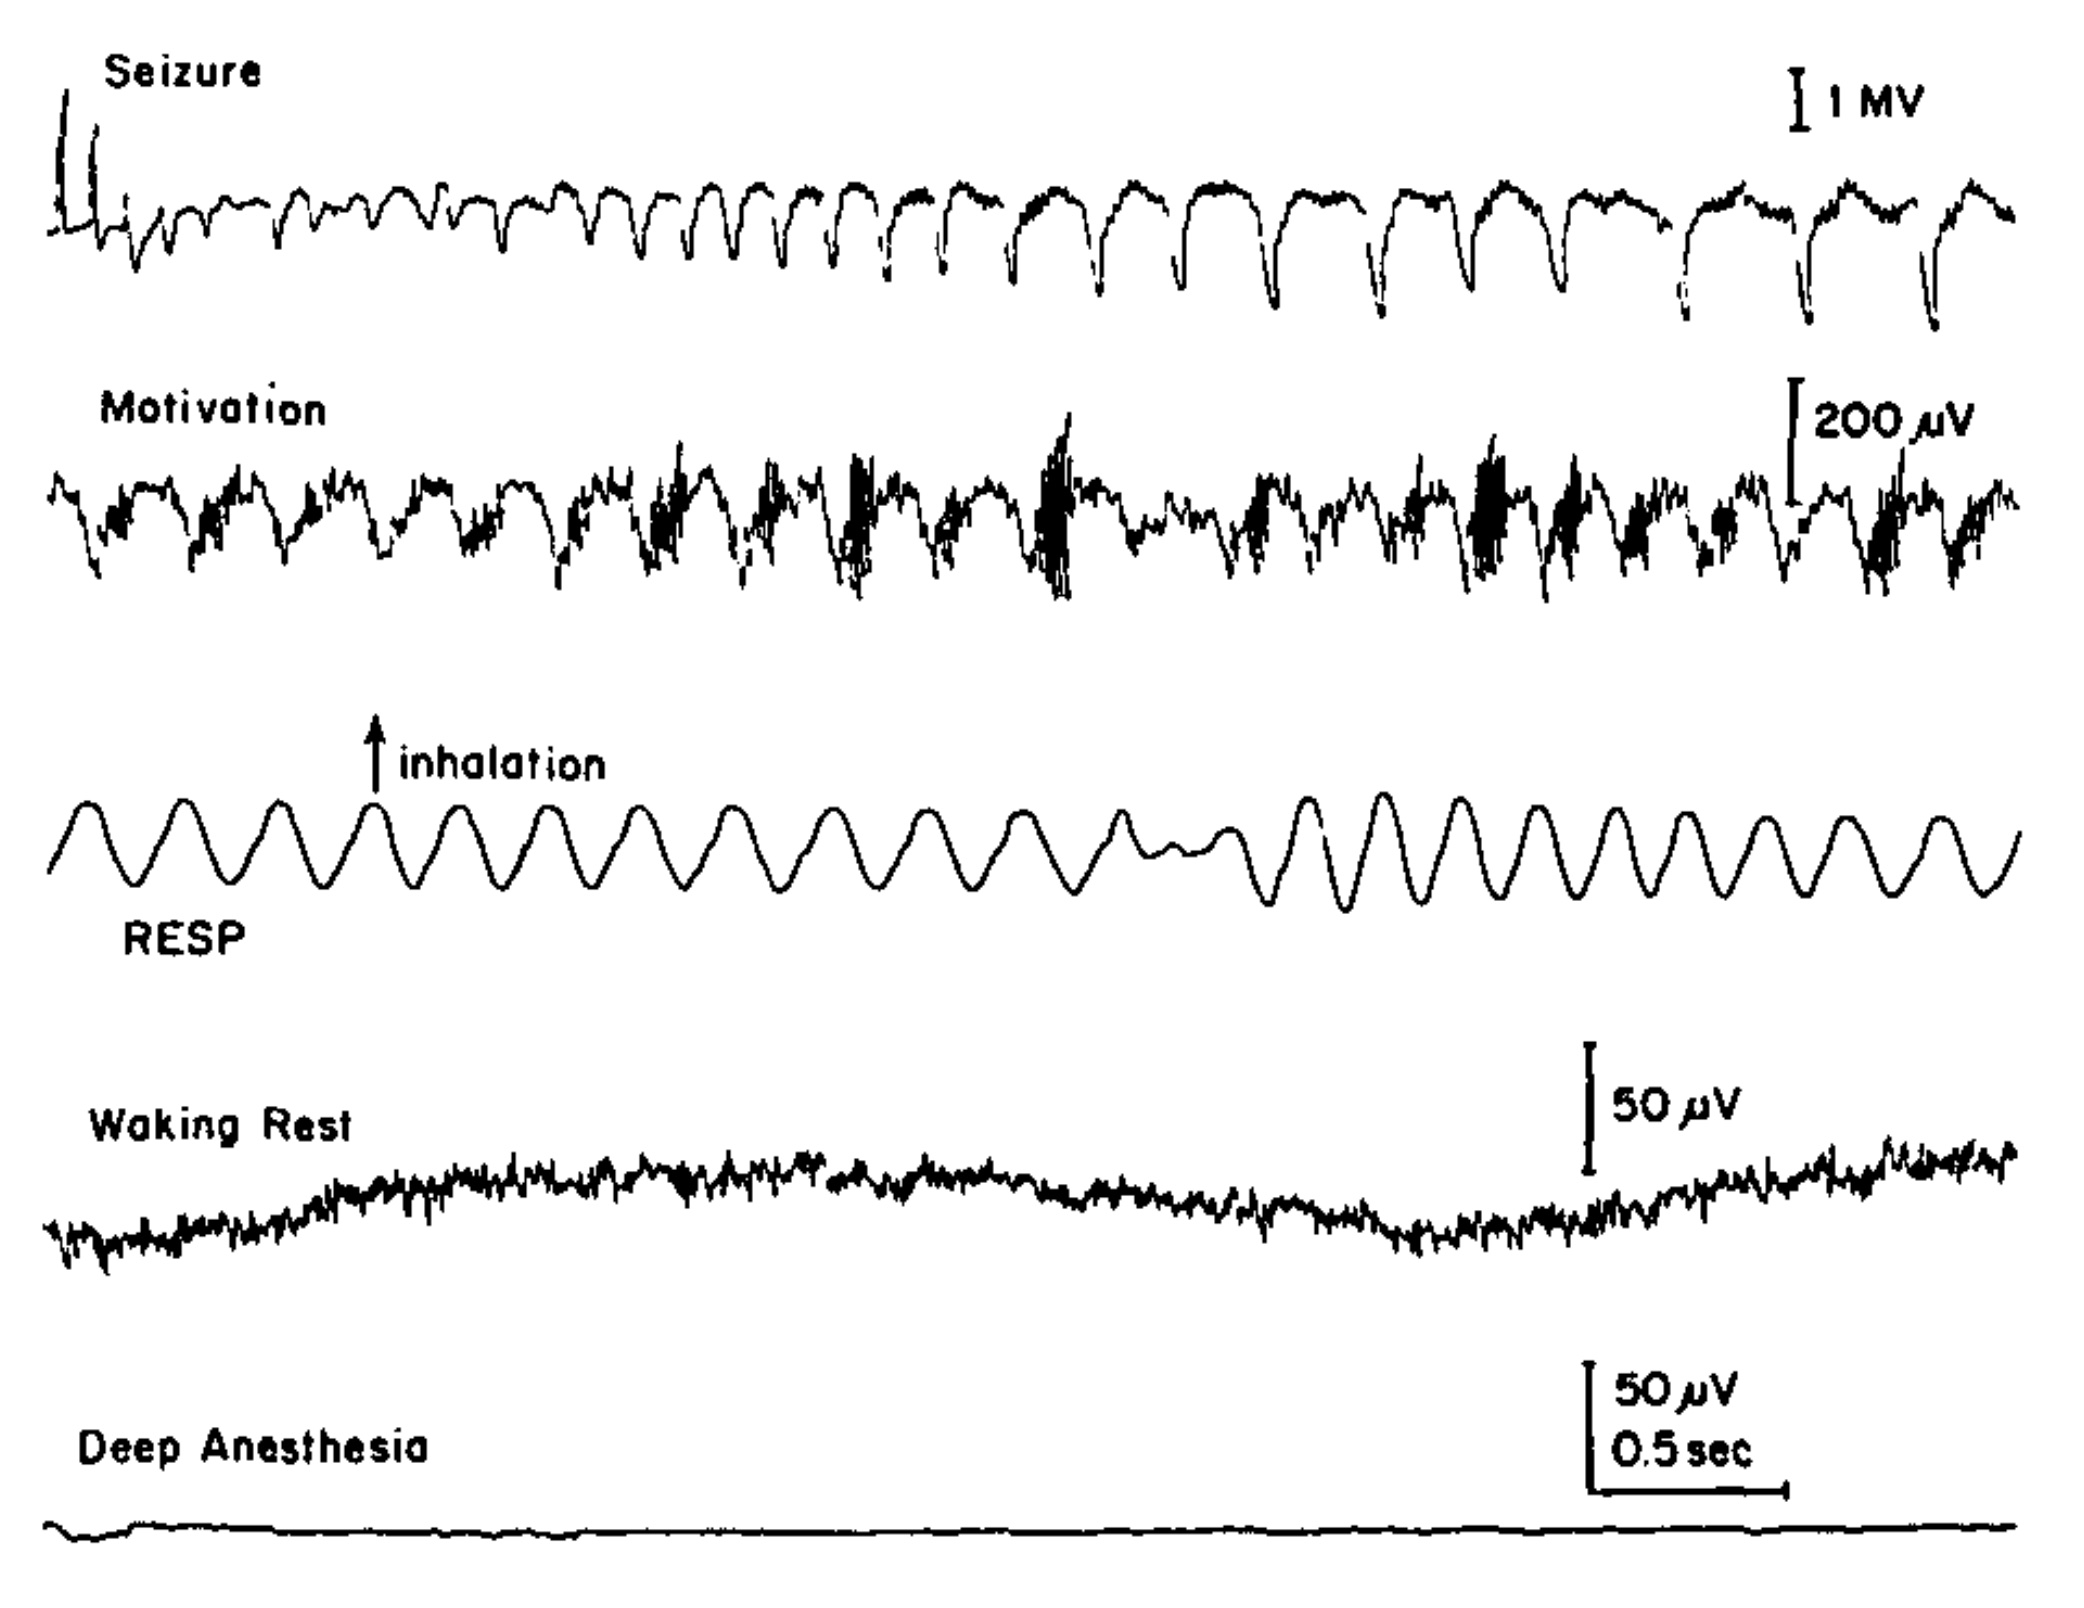
\includegraphics[height=3.5in]{images/fig2.jpg}
    \longcaption{从脑电图轨迹中识别出嗅觉系统的四种状态}{在深度麻醉下(最低的轨迹),波动被压制。在清醒但未受到激励的动物中,振幅较低,轨迹表现不规则且难以预测。在受到激励时,不规则活动被气味刺激吸入时受体激活的嗅球的短暂振荡爆发中断。在对侧嗅道(LOT)进行几秒钟的强烈电刺激(最上方轨迹)下,可诱发癫痫发作。癫痫的发作始于激发性输入传输的失败,如左侧对刺激序列最后五个脉冲的递减反应所示。随后,癫痫尖峰列逐渐从刺激后相对平静的状态中显现出来。摘自 Freeman (1987a)。}
\end{figure}

嗅球脑电图空间频谱的测量(Freeman 1980;Freeman \& Baird,即将发表)用于确定电极阵列间最佳间隔(空间数字化增量)为0.5毫米,相当于奈奎斯特频率1.0 c/mm。一个8×8阵列在考虑到64个通道的限制下,提供了一个大约3.5×3.5毫米的嗅球“窗口”。对兔子EEG的时间频谱测量表明,最感兴趣的频率范围是20-90赫兹。滤波器设置在10和160赫兹,时间数字化增量为2毫秒,对应奈奎斯特频率250赫兹。选择了76毫秒作为单次吸入对嗅球反应的最短持续时间,因此对气味剂或对照背景空气吸入的单次事件的单次未平均测量包括64×38个时间值,以12位进行数字化,并保留了8个最重要的位。每次试验产生3个对照事件和3个测试气味事件。每次会话进行了10次CS+和10次CS-试验,共120个事件。这项研究的数据基础包括5只兔子在熟悉期后进行的18次会话。

收集这些数据需要64个前置放大器、一个高速多路复用器和模数转换器(ADC),以及一台专用计算机(Perkin Elmer 3220)和硬盘。数据采集的限制因素最终被证实是在6秒的试验期间核心到硬盘的数据传输率,以及双缓冲处理。我们设计了一些程序用于离线编辑和排除干扰(Freeman \& Schneider 1982)、时间滤波和分解(Freeman \& Viana Di Prisco 1986b)、空间滤波和反卷积(Freeman 1980;Freeman \& Baird,即将发表)以及对测量结果进行多变量统计分析(Freeman \& Grajski,即将发表;Grajski, Breiman, Viana Di Prisco \& Freeman,即将发表)。这些程序在其他文献中有详细的回顾(Freeman 1987b)。

\begin{figure}[ht]
    \centering
    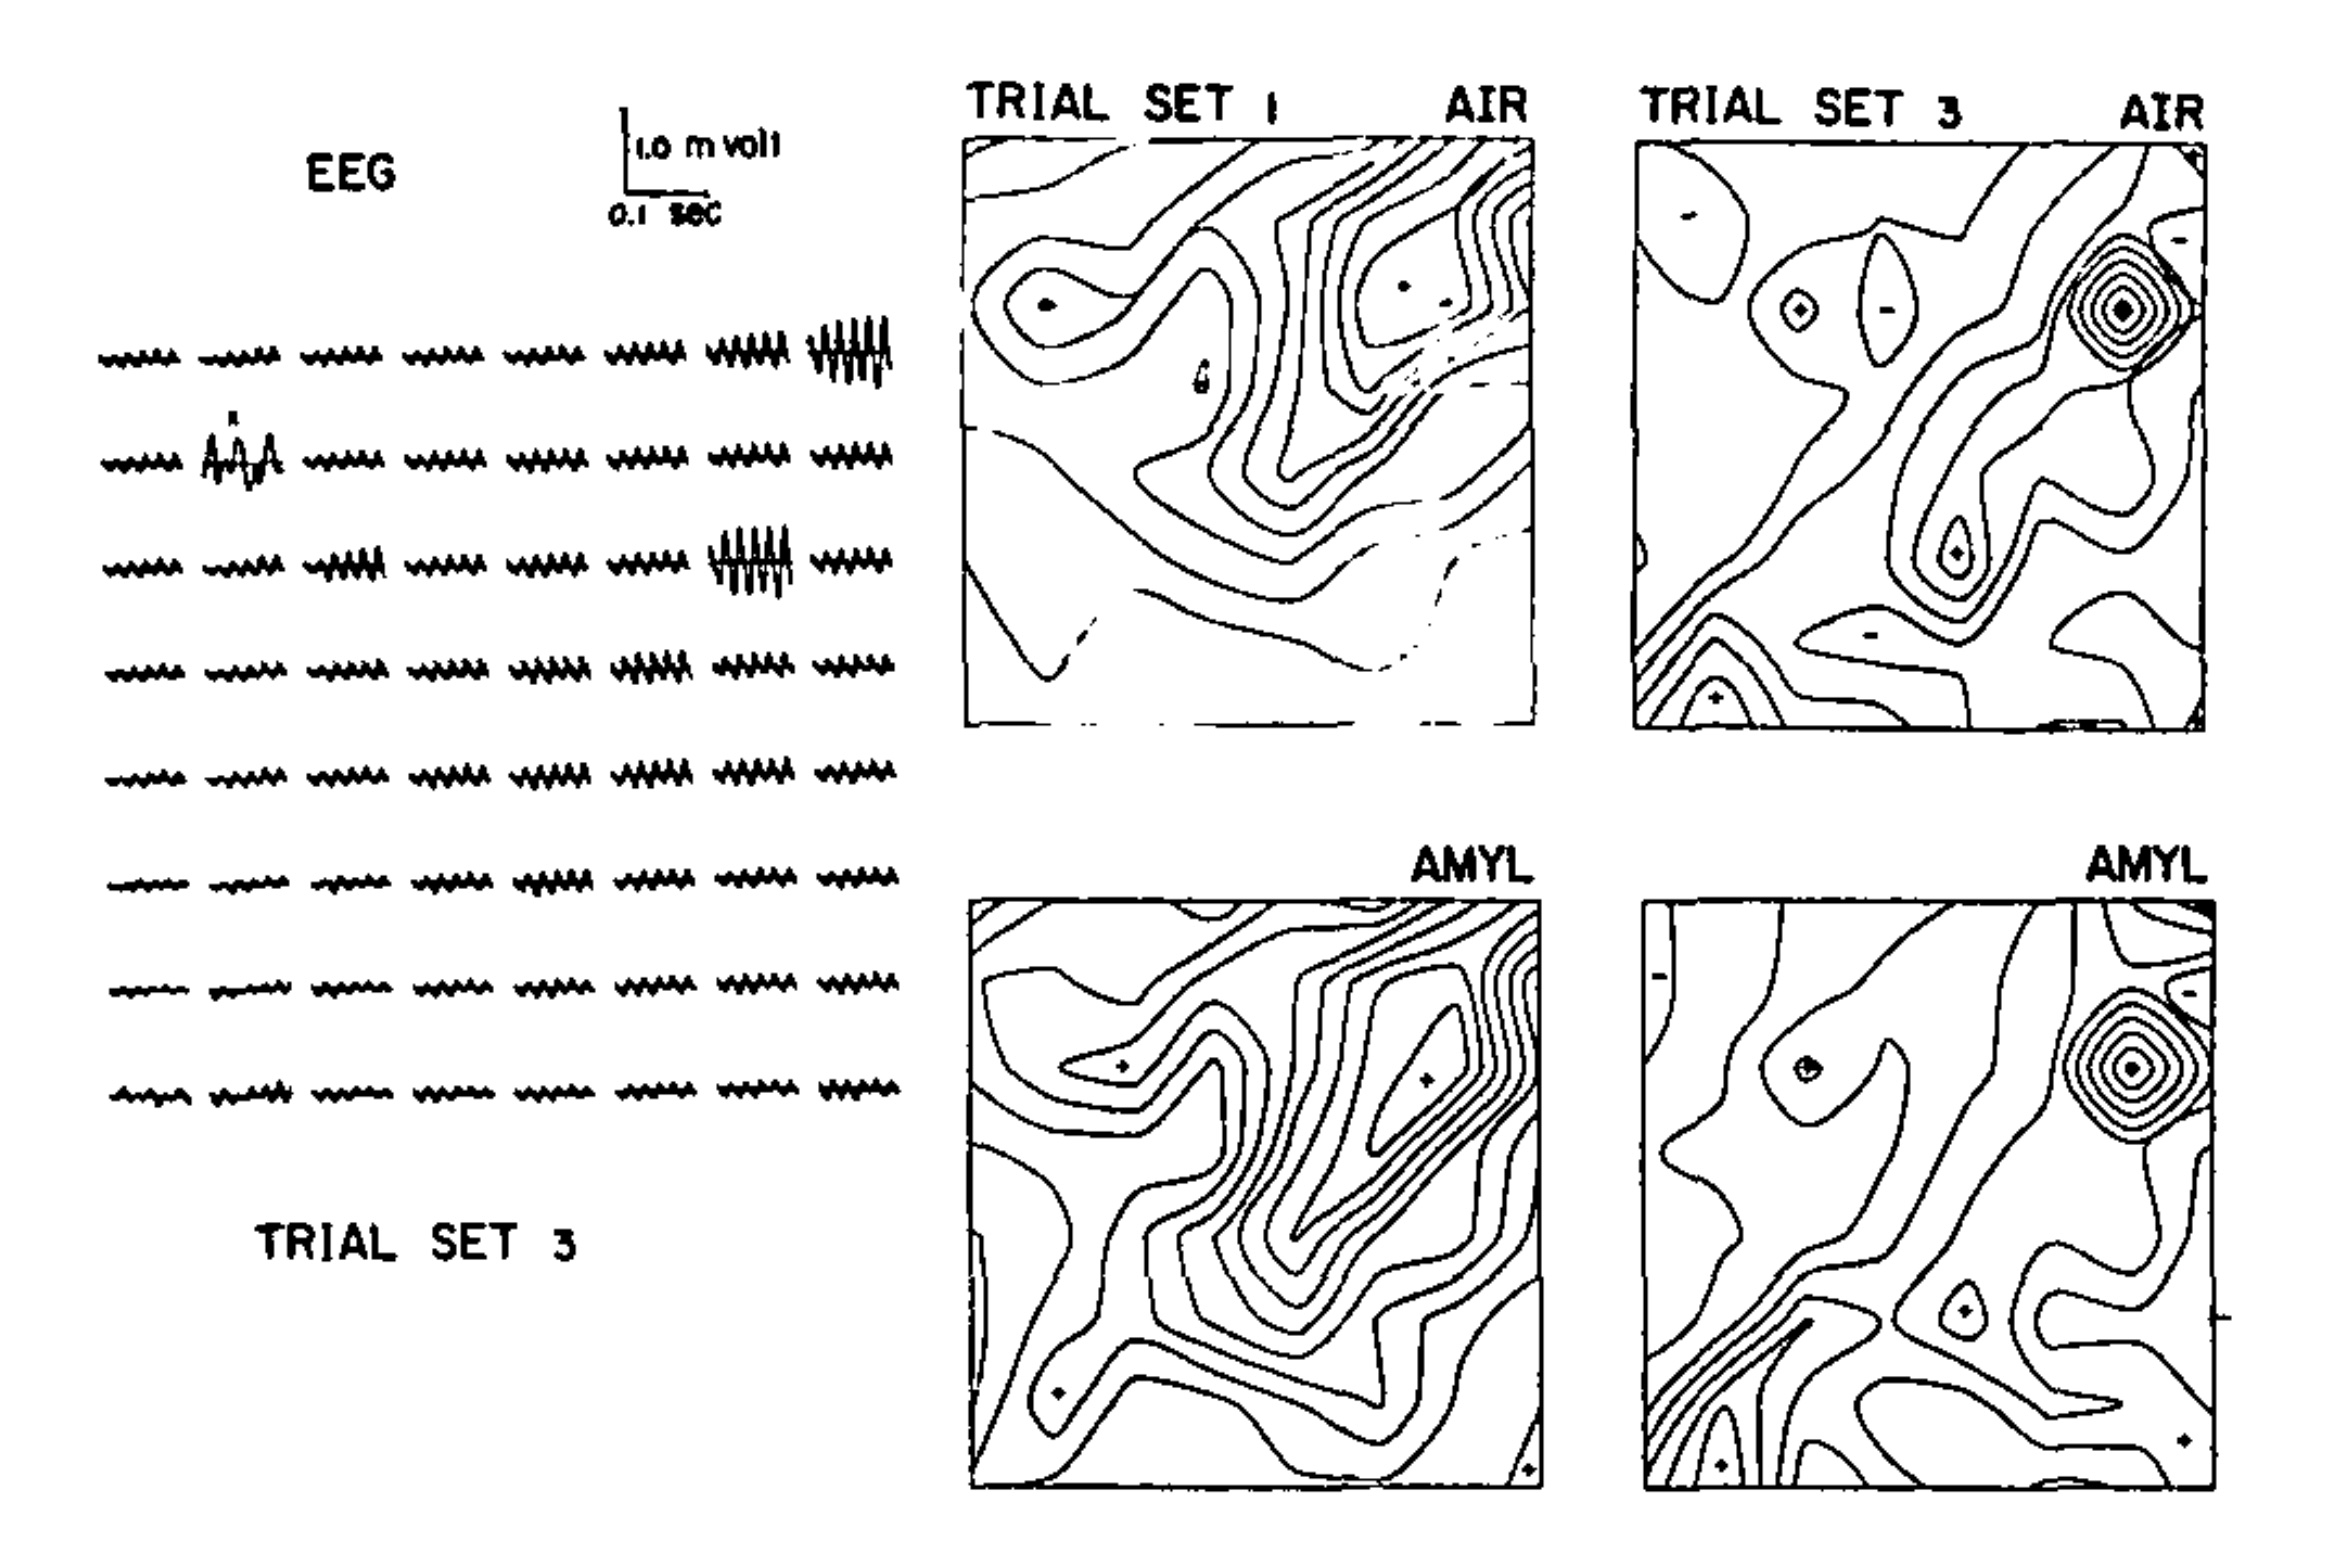
\includegraphics[height=3.5in]{images/fig3.jpg}
    \longcaption{未平均脑电图轨迹}{左图展示了一组单次未平均的脑电图轨迹,这是来自一次试验组中10次爆发的一次气味爆发。图中的“(x)”标记了一个坏通道记录的例子,在编辑过程中用两个相邻记录的平均值进行了替代。右图:对比了没有气味(上图,“空气”)和有气味(下图,“戊酸乙酯”)时的爆发的均方根振幅。左边的两种模式之间存在显著差异,但右边的两种模式之间则没有。摘自 Freeman and Schneider (1982)。}
\end{figure}

测量过程包括对每个事件中的64条信号轨迹进行曲线拟合。我们识别出5种基本波形或基础函数,这些函数在所有64条轨迹中以不同程度共有。通过回归分析,将这5个基础函数的总和拟合到每条轨迹上,生成了5个矩阵,每个矩阵包含64个幅度值,这些幅度值共同包含了事件总方差的80\%,同时也生成了残差矩阵和高通及低通数字滤波的两个残差矩阵,所有这些均以均方根幅度表示。评估过程包括确定这8个矩阵中哪些最能(或是否能)根据CS和CR正确分类事件。在进行这种测试之前,不会丢弃任何数据。此外,还检查了基础函数的系数,以确定它们是否包含特定于气味剂的信息。

最终结果是非常明确的。主导基函数的幅度矩阵——即那个包含总功率最大部分的基函数的幅度矩阵——足以正确分类事件。这些矩阵在4只兔子中的5只对两种气味剂的分类准确性远高于偶然水平,这些兔子在行为上能区分这两种气味,但第五只兔子未能区分它们,因此没有从这只兔子记录到的事件(Freeman \& Grajski,即将发表;Freeman \& Viana Di Prisco 1986b;Grajski et al.,即将发表)。

图3展示了一个事件的例子(未平均轨迹)。每条轨迹的关键属性是它们都具有相同的时间波形。异常情况通常是由于干扰或电极未放置在嗅球上。通道间的振幅不同,形成了一个空间模式,这个模式(平均来说)相对稳定,且每个动物都能容易识别。在熟悉之后,这些振幅模式保持不变,除非进行了气味剂条件反射训练。新模式只与强化气味剂相关联出现,而不是仅与视觉或听觉的CS或UCS相关联。只要S-R(刺激-反应)条件保持不变,它们在会话内和会话间都保持稳定。

在区分性条件反射训练下,出现了多种模式。当引入一种新的气味剂CS+,或者将先前的CS+变为CS-时,整套空间模式似乎都发生了变化。在涉及改变S-R条件的不同阶段之间的变化量,以总的跨会话、会话内阶段方差的一部分来衡量时,相对较小(7%)。这些稳定的空间模式中的信息,用于根据CS和CR正确分类事件,不局限于特定的通道子集。换句话说,信息密度(与内容不同)在空间上是均匀分布的,就像印刷页面上的字母间隔一样,无论它包含字母、标点符号还是根本没有字符都具有相同的价值。

\subsection{背景活动的出现}

\begin{figure}[ht]
    \centering
    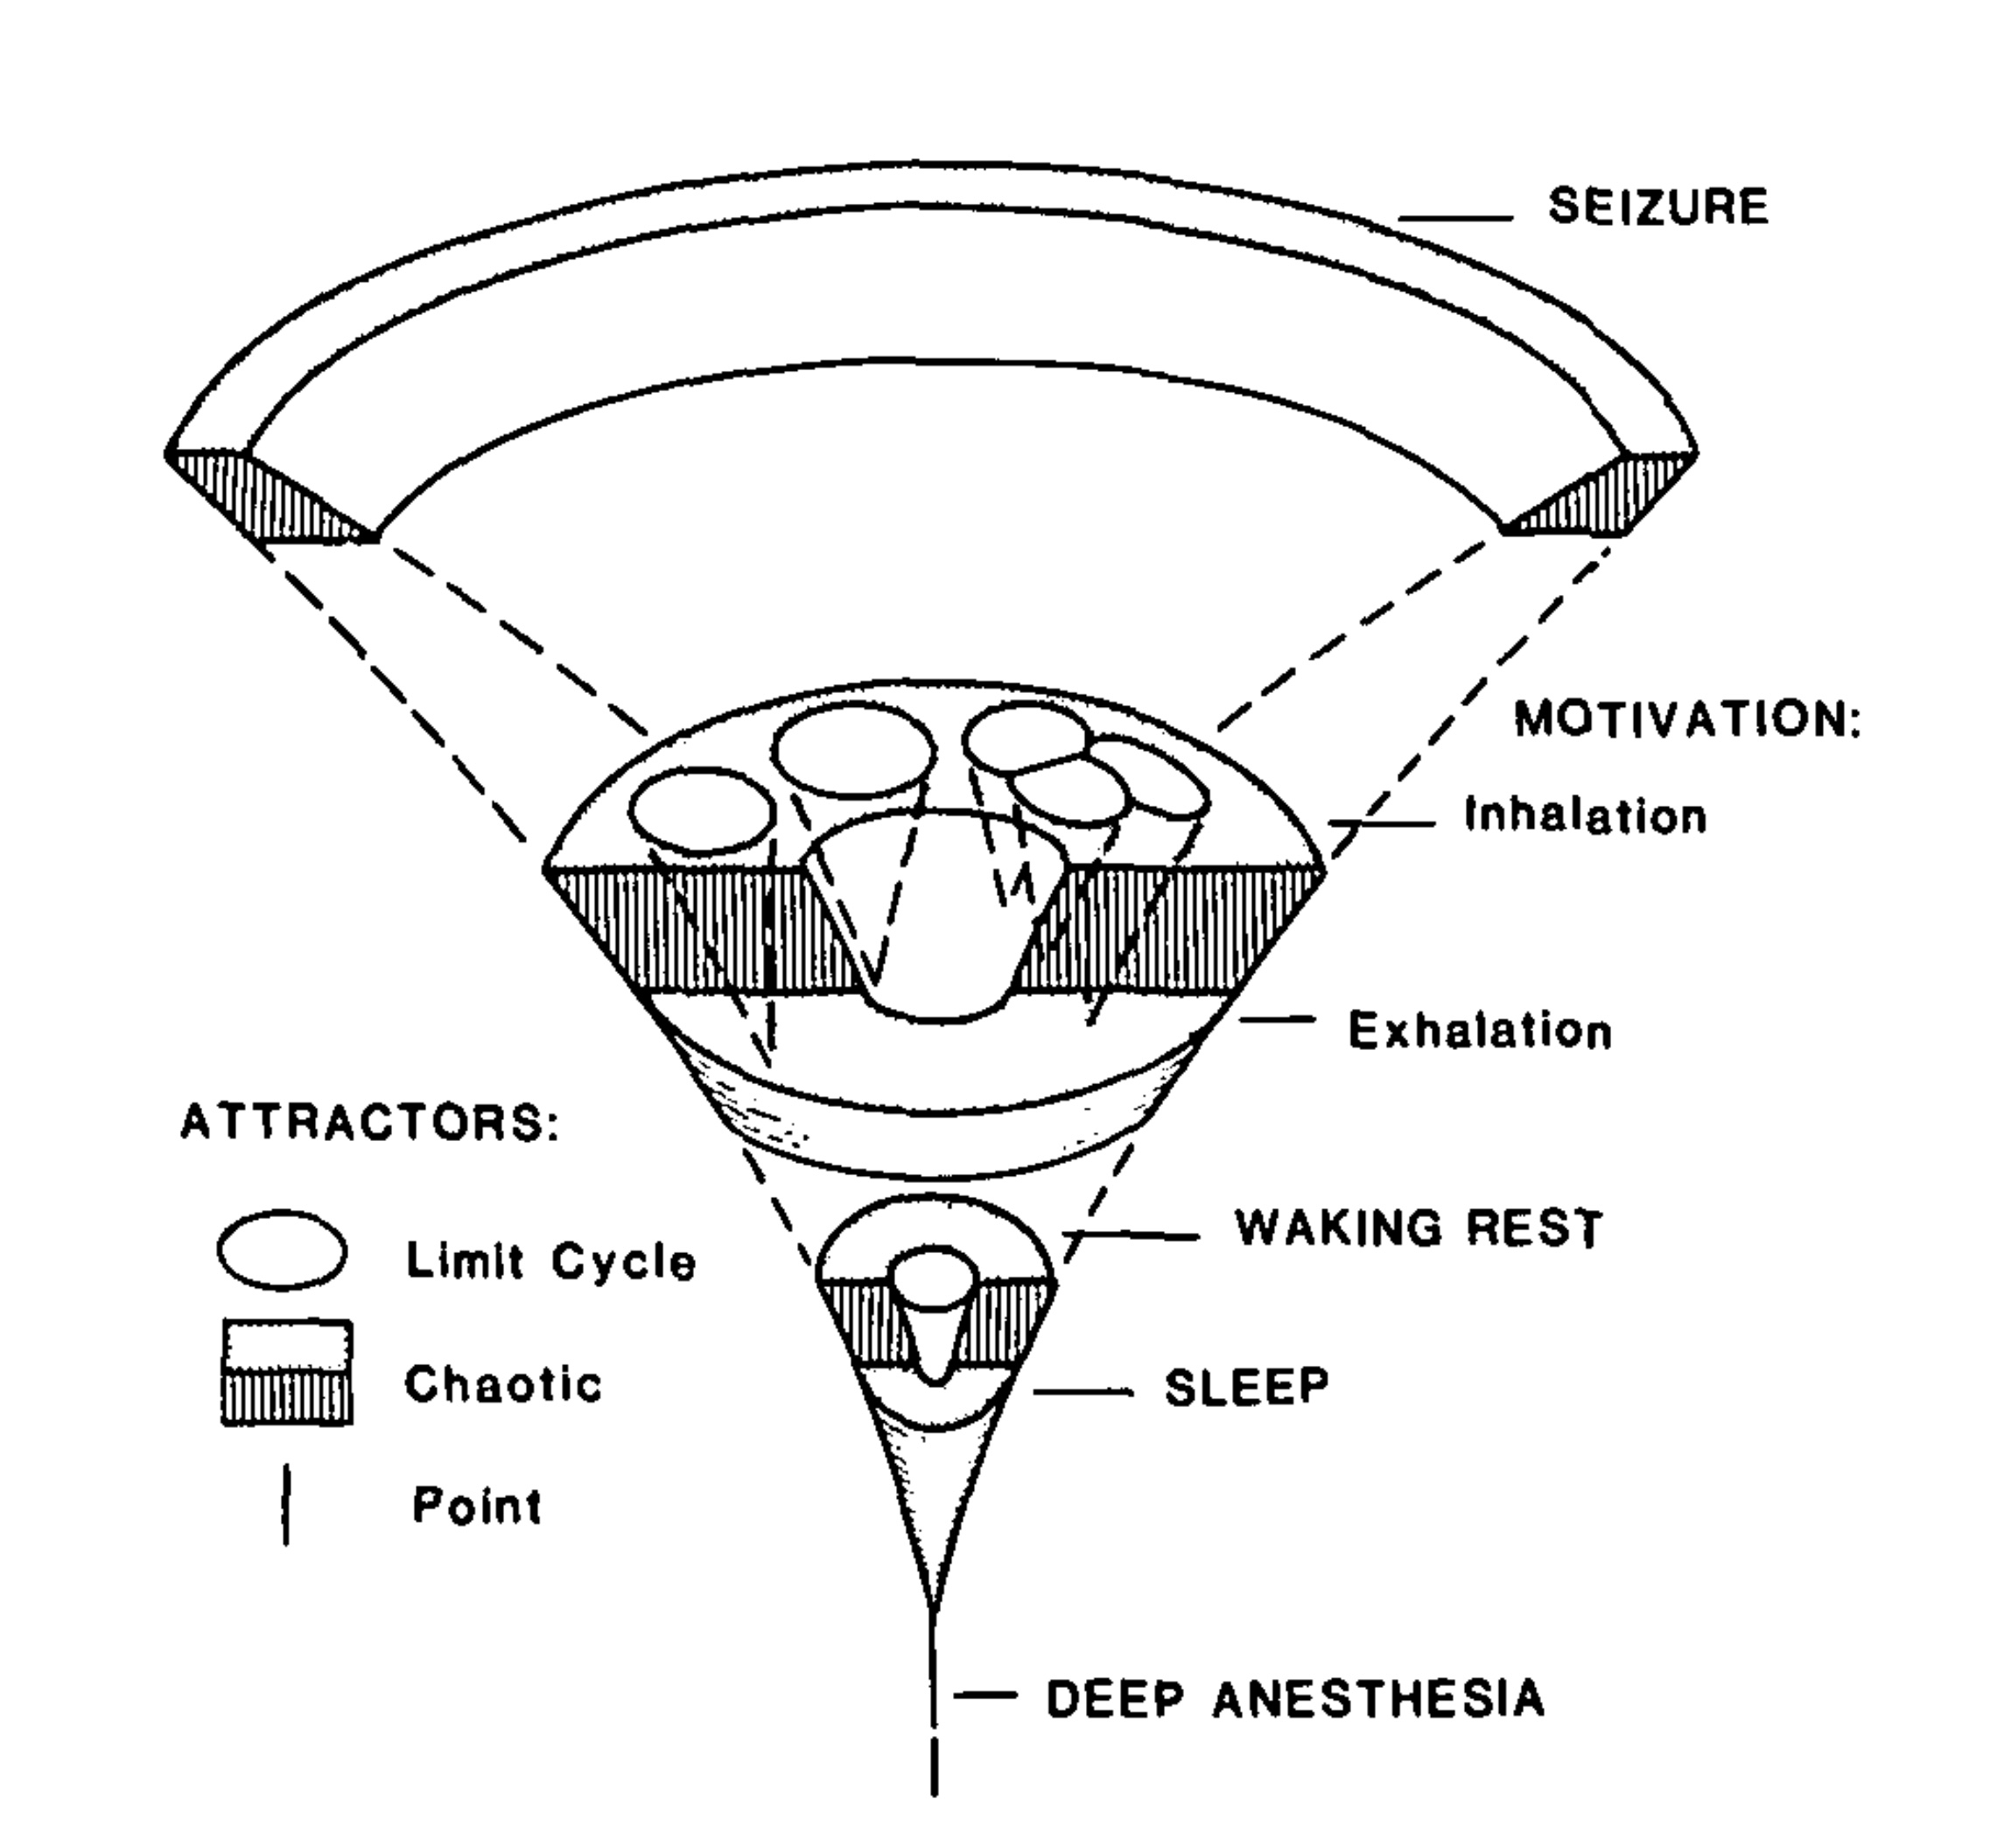
\includegraphics[height=4.5in]{images/fig4.jpg}
    \longcaption{}{这个瓶状结构试图展示嗅觉动力学的状态空间图。两个水平方向的维度分别代表激动性子系统和抑制性子系统活动的幅度。垂直轴用于表示一个分叉参数,即对这两个子系统的平均驱动输入水平,包括来自向心激活受体的输入和与唤醒及动机相关的离心投射输入。最底部的线表示一种平衡状态或点吸引子。阴影区域代表混沌吸引子,而空心圆表示极限环吸引子。每个阶段的活动情况在图2中有所展示。基于这个图表制作的相位图在图11中展示。摘自 Freeman (1987a)。}
\end{figure}

我们认为,这是首次证明在大脑皮层任何部位的 EEG 活动的空间维度中存在感觉和运动特定信息。之前没有展示这一点,是因为在该项目的所有层面都面临着问题。这些问题包括实际问题,如阵列的设计和制造、外科植入手术、控制和测量兔子的行为、管理每次试验约1.2亿比特以及每个实验系列数十亿比特的数据流,以及在体积传导分析、统计力学、非平衡热力学、非线性动力学和应用于神经活动的多变量统计学等不同领域的基本理论问题。制造电极阵列、磁力拾取器或光学探头及其前置放大器仅仅是为数据的大量流入做准备。真正的难题在于适应正常和学习行为的记录条件,以及合理设计数据降维和精炼的算法。我们的方法恰好是第一个取得成功的方法;由于没有先例,我们没有其他数据可以与我们的结果进行比较。就像我们在数据获取方面的开创性工作一样,现在我们必须在理解这些数据关于大脑功能的含义方面继续探索新领域。

在嗅觉研究中,正如在所有大脑生理学中一样,我们必须处理的基本现象是在“自发”脑电图(见图2)和整个中枢神经系统(CNS)神经元单位活动中表现出来的背景活动。这种活动是如何产生的,它起着什么作用?这种活动极其稳健;除了最严重的脑组织伤害,如近致命的麻醉、缺血或缺氧,它几乎可以在所有情况下存活下来。也许唯一可靠的抑制方法,且不会杀死组织,是通过手术分离出小块皮层(Burns 1958),切断神经连接,同时保留血液供应(即使这样,活动也可能不会完全消失)。这种手术对嗅球和前梨状皮层同样有效(Freeman 1986),前提是它们与彼此以及与受体和大脑的其余部分隔离开。在完全手术切断神经连接但仍保持足够供血以维持生存的情况下,每个结构都会变得“沉默”,除非受到电刺激或化学刺激。当受到干扰后放置不管时,每个结构都会产生反应,然后再次变得沉默。通过平均诱发电位(AEPs)和动作电位的刺激后时间直方图(PSTHs),可以观察到对电脉冲刺激的反应。

动态结构是否稳定,取决于系统在经历扰动后能否恢复到原先的状态。如果这个基础状态既稳定又不发生振荡,我们就说这个系统达到了平衡。当我们在图表上绘制振幅或能量的值时,这些值相互对应,形成的响应曲线或轨迹会在系统达到平衡时收敛于某一点。无论起始条件如何变化,在扰动影响下,系统都会趋向于这一相同的点。因此,这个点被称作“吸引子”,而所有可能导致系统达到这个吸引子的起始条件集合,被定义为这个吸引子的“盆地”(见图4)。当我们通过控制系统输入将其置于某个吸引子的盆地时,这时的系统动力学就被认为是受该吸引子控制的。

当通过深度麻醉(Freeman 1986)或冷冻阻断嗅球和前梨状皮层间的轴突连接(Gray 1986)来诱导灯泡(见图2,底部轨迹)或大脑皮层达到稳定平衡状态时,这种状态是可逆的。随着系统的恢复,背景活动也会重新出现。这时,系统可以说是发生了“分叉”,进入了一种新的状态,原来的点吸引子被点排斥子所取代(见图4)。当尝试抑制或限制活动失败或仅仅短暂成功时,就会出现排斥子的现象。嗅球和前梨状皮层这两个互相连接的结构无法保持平衡,它们必须持续活动,即使它们只与彼此相连,而不与大脑的其他部分相连(Freeman 1987a)。当系统在其动态过程中经历重大转变时,例如从睡眠到清醒,或从正常状态到癫痫活动,就会发生一种分叉。控制这些过程的方程式是相同的,但其解决方案却发生了根本性的变化。我们认为,系统动态的控制从点吸引子转移到了混沌吸引子。这意味着系统进入了一种不稳定但有限的活动状态。从统计学意义上讲,这种状态是固定的,但其数学特性与“噪声”(Grassberger \& Procaccia 1983)不同。

这种背景活动从统计学角度看与我们所说的带限噪声没有区别,也就是经过带通滤波器处理的白噪声。多年来,我们已经知道来自单个神经元的尖峰列的时间间隔直方图符合有不应期的泊松过程,因此我们推测背景脑电波是反映或控制着这些尖峰列的树突电位的局部平均值,类似于“布朗运动”。这一假设似乎得到了验证,因为记录点之间的距离越远,两个轨迹之间的相关系数就越低。然而,根据我们最近的研究,我们现在知道这种观点是错误的。不管波形看起来多么“嘈杂”,嗅球脑电波活动的瞬时频率始终保持一致。相关性与距离成反比是因为覆盖整个嗅球的小但系统性的相位梯度(Freeman \& Baird,即将发表),而不是样本之间的统计独立性。波形的共性不会扩展到嗅球之外,但在嗅球内部几毫米的范围内是有的,这个范围远远超出了体积传导所能解释的。嗅球脑电波是由嗅球内部密集的反馈互动产生的全局特性,而这种特性又受到嗅球外部反馈互动的影响。

\subsection{混沌的证据}

对背景活动的神经机制的解释源于我们使用 Grassberger-Procaccia (1983)算法来测量我们动物休息时持续脑电图样本的自由度(豪斯多夫维数)。初步估计介于4到7之间(Freeman 1987b),表明该活动反映的不是“噪声”,而是混沌(见注释1)。这个关键区别类似于棒球比赛中人群的噪声和家庭争吵的噪声之间的差异。混沌在外观和统计特性上与随机噪声无法区分,但它是确定性的,而不是随机的(Garfinkel 1983; Rössler 1983)。它具有相对较小的自由度;它可以通过分叉(见第3.2节)几乎瞬间开启或关闭,就像开关一样,不像热噪声那样需要相对缓慢的加热和冷却。混沌是受控制的噪声,具有精确定义的属性。任何需要随机活动的系统都可以从混沌发生器中比从噪声源中更便宜、更可靠地获得它。甚至数字计算机的随机数生成器也是混沌算法;给定相同的种子,随机数序列被精确地复制。

为了模拟嗅觉系统的脑电图,我们采用了一系列非线性常微分方程。这些方程之前分别用于模拟嗅球、前嗅核(AON)以及前香皮质(PC),并且关注于它们的平均诱发电位(见图5)。我们将这些方程组合成一个相互作用的网络(见图6)。通过精确调整反馈增益和分布延迟,以适应我们对整个系统解剖和生理学的了解,我们的模型成功模拟出了与休息状态动物的背景脑电图在统计上无法区分的持续混沌活动(见图7)。在模拟感受器输入的条件下,该模型还能生成类似于嗅觉EEG在吸气时观察到的“爆发”式振荡事件(见图8)。

通过对嗅球和前嗅核(AON)之间的增益进行微调,我们的模型系统进入了一种退化状态,其豪斯多夫维数接近2,并呈现出重复的尖峰(见图2),这与电刺激引起的嗅觉癫痫中的癫痫形尖波列极为相似(见图9)。这一现象为我们提供了从稳定点吸引子向混沌吸引子转变的研究手段(Babloyantz 和 Destexhe, 1986)(见图4)。我们通过在模型中增加兴奋性增益连接来实现这一点(见图10中的App,以及图6中P和M集合之间的连接)。这导致了Ruelle-Takens-Newhouse引导至混沌的路径(Schuster, 1984)。在模型的“癫痫”状态下,其混沌吸引子是一个2-环面;而正常状态下的超混沌背景活动的混沌吸引子维度更高,其几何结构仍是未知之谜。这些结果,代表了正常和异常脑电图活动的首次成功模拟,并且相关的实验证据支持这一数学模型(Freeman, 1987a),在其他文献中有详细论述(Freeman, 1986)。

考虑到这个神经系统动力学的整体情况(见图2、3和4),我们可以用相位图像来形象地描绘其多个稳定状态。如图11所示,每个状态都可以表示为一个在两个维度上的表面:一个维度是代表性的局部兴奋神经元群体的活动水平(左-右轴),另一个维度是抑制神经元群体的活动水平(进出纸面的轴)。每个位置的垂直高度代表该点活跃状态的能量量。诱发电位看起来像是一个逆时针方向的螺旋轨迹;而背景活动则像是围绕中央突起底部的不规则圆形涂鸦。深麻醉状态的平衡点在最底部的最低板上。它的最低点是点吸引子。从一个状态向上转移到下一个状态取决于系统内部交互的程度(即分岔参数),这受到模型中多个参数以及大脑对输入和觉醒条件的影响。通向清醒但无动机状态的分岔序列是通过中央隆起的出现,一个点排斥器的形成,以及围绕其的包含混沌吸引子的井的形成。中央隆起引发的状态变化实现了从点吸引子向混沌吸引子的控制转移(见图4)。

如图11所示,嗅觉系统及其相应的模型表现出多个层次的状态。尽管基本的神经动力学和方程在所有状态中都是相同的,但系统的行为会根据不同的神经条件和模型参数而有所不同(例如,在清醒、睡眠、爆发、间爆发间隔、癫痫等不同状态下)。这两个系统都有能力进行突然的、剧烈的、全面的从一种状态跳跃到另一种状态。这些就是所谓的分岔。这些分岔在本质上类似于物理系统中的相变,比如冰变水,水变蒸汽。分岔有许多不同的形式和种类,因此很难甚至不可能给出一个确切的定义。

\subsection{混沌在气味识别中的作用}

混沌在气味识别中扮演着重要角色。随着动机的增强(如食物或水剥夺),这种配置得以维持,使背景活动的振幅增加,但这种现象只出现在晚期呼气阶段。在晚期吸气和早期呼气时,感受器输入激增,进入嗅球,使嗅细胞去极化,增强嗅球的敏感性,并引发振荡爆发。这是从低能量混沌状态向高能量、能量分布频谱狭窄的状态的转变,表明它受到极限环吸引子的控制。从混沌中涌现出秩序的两个方面是:首先,出现了狭窄的频谱峰,显示出高度的时间相干性。其次,振荡的局部振幅与特定气味物质(作为条件刺激CS)的关系固定。不同气味的振幅不同,说明存在多个极限环吸引子,每种气味对应一个,每个都导致爆发中的规律振荡。

正如图11中所假设的,这些吸引子在晚期呼气和缺乏动机的情况下是潜在的。它们会在有动机的每次吸气时重新出现,随着呼气消失。我们推测,在吸气时选择一个吸引子是由于吸入空气中存在特定的条件刺激(CS)气味或没有气味,从而选择一个与背景气味或行为现状相符的吸引子。换句话说,特定受体群的化学刺激会在吸引子在分岔过程中出现时,将系统置于特定的状态中。随着呼气,系统回到基础状态,为处理吸入空气中的新气味样本信息做准备。混沌吸引子的主导作用可能在所有层面上都紧密相关,它从休息的低能量状态延伸到高能量的癫痫状态。我们推测,混沌活动提供了一种锻炼神经元的方式,这种方式保证不会导致周期性固定或空间结构化活动(Conrad 1986)。它还允许在每次吸气时迅速而公平地访问每个极限环吸引子,确保动物随时可以即时访问其所有已学习的区分信息。无需通过记忆库进行搜索。此外,吸气时的混沌井也是一种安全网,用于机制未能收敛到已知吸引子的情况,可能是因为样本不足或吸入空气中存在新颖或不熟悉的气味。在这两种情况下,都会产生一种特征为频率调制过度、峰值频率较低、时间频谱广泛的“混乱”或混沌爆发。尽管波形在空间上共享,但这些爆发并不会收敛到一致的空间振幅调制模式,除非通过重复强化呈现形成新的CS和新的CR,这种情况下会出现新的极限环吸引子。换句话说,混沌井提供了从所有已建立的吸引子中逃脱的途径,使动物能够将气味分类为“新奇”,而不比对任何已知样本的分类更延迟,并且它获得了在构建新吸引子时保持非结构化活动的自由。

因此,在我们的观点中,混沌在系统中发挥着几个关键作用。这个系统被设计和构建的目的是为了确保其自身拥有一个稳定且受控的“噪声”来源(即混沌)。最引人注目的是,当机制启动信号时,它会关闭混沌,因此“信号”并不是在混沌中被检测到。EEC对创伤的免疫性表明,这种机制非常稳定,但并不是绝对稳定。小发作型癫痫(见图2)发生在反馈控制系统因过度电刺激而超出正常范围,并发展出动态不对称时。这种不平衡导致了一种病理性不稳定性,暂时将系统带入一个退化的、低维度的混沌活动状态;其模式类似于在深麻醉后从“沉默”状态恢复的早期阶段所见的EEC尖峰活动。我们认为,这种常见的癫痫形式显示出了一个“阿喀琉斯之踵”,即大脑感知器官的各种混沌形式的产生和维持的普遍且广泛的神经机制的本质地基状态。

\subsection{学习和神经元细胞集合}

形成新极限环吸引子背后的神经机制的变化已在其他地方进行了详细的描述和讨论(Freeman 1975; 1979a-c; 1981; 1983b)。我们的模型基于对嗅觉系统中电刺激作为条件刺激(CS+)或非条件刺激(CS-)时平均诱发电位波形变化的研究,以及通过模拟嗅球或皮层动力学的微分方程冲激响应解来复制这些波形。简单来说,这些结构中的兴奋性神经元通过轴突侧支相互连接,在双向突触中主要连接于细胞体(Willey 1973)。当这些神经元由CS+成对共同激活时,它们的联合突触会按照赫布规则得到加强(Viana Di Prisco 1984)。所需的强化是通过去甲肾上腺素介导的,由蓝斑核释放到嗅球和皮层(以及其他部位)(Gray 1986; Gray, Freeman \& Skinner, 1986)。我们的模型显示,突触强度的适度增加25-40\%可以使嗅球对CS+的敏感度增加40,000倍(Freeman 1979a; 1979b)。

通过加强兴奋性突触将选定的神经元子集(可能仅占总数的1-5\%)链接起来,形成了神经细胞集合(NCA)。此后,任何部分的兴奋都倾向于扩散并激活整个集合。我们设想,每个NCA存在于嗅球中,它们像面包上生长的霉菌一样形成丝状网络。我们推测,激活特定NCA的一些神经元将选择吸引子的盆地,而在吸气时,嗅球机制就会向这个盆地汇聚。

理解这种开关装置的关键在于理解控制在互动质量中神经元行为的静态非线性。在没有输入的情况下,神经元倾向于活动低于阈值并保持静默。在持续激励下,它们会产生稳定的输出。由于动作电位的离子机制,在接近阈值的动态范围内,形成动作电位的倾向随着去极化呈指数增加。动作电位释放的恢复性力量可以限制射频率,但这种作用可以说是事后的。


\newpage
\phantomsection
\addcontentsline{toc}{section}{参考文献}
\bibliographystyle{abbrv}
\bibliography{data/reference}

\end{document}


